\centerline{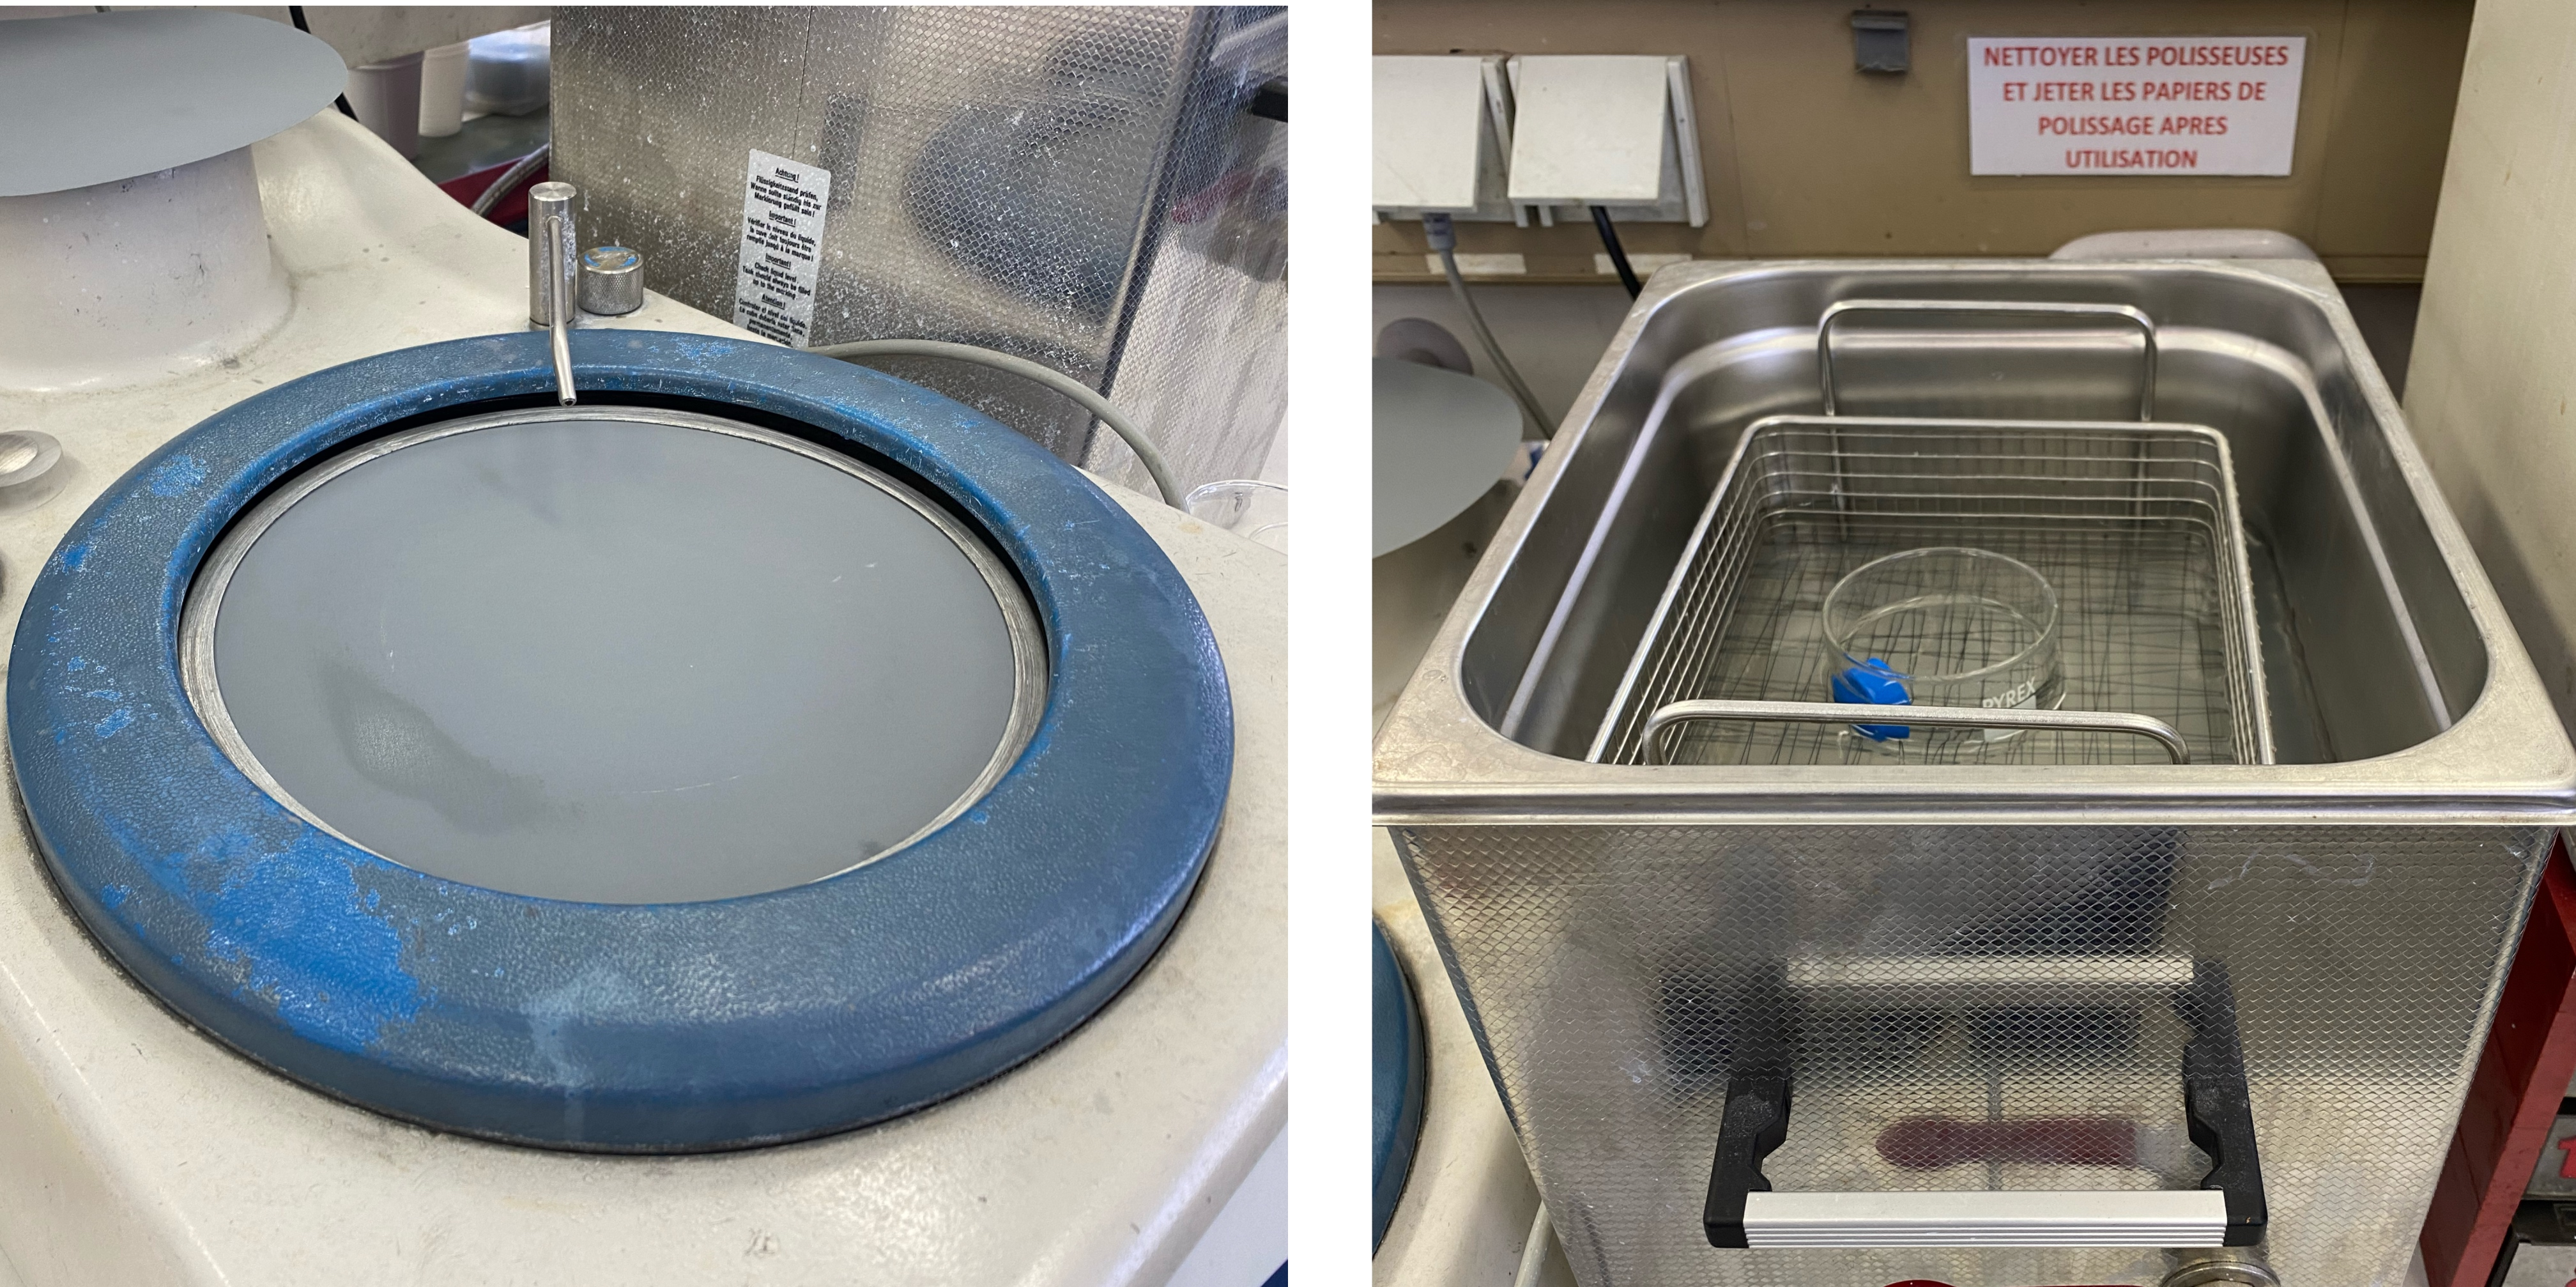
\includegraphics[width=0.55\textwidth]{images/WechatIMG1126.jpeg}}

\\\\
L'étape de polissage et nettoyage est cruciale pour ne pas avoir 
trop de défauts à la surface de l'échantillon:
on polit la pièce sur un polisseur tournant (1200 -> 2400 (eau)), puis on la passe au bain à ultrasons 2 minutes pour la nettoyer.
Ensuite on fait le passage à 2µm et 1µm (lubrifiant),
puis on la repasse au bain à ultrasons.\\
\\
\\
\centerline{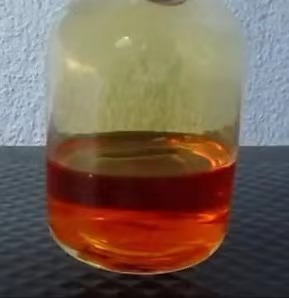
\includegraphics[width=0.35\textwidth]{images/WechatIMG1128.jpeg}}
\\
On utilise un mélange composé de deux tiers d'acide chlorhydrique 
et d'un tiers d'acide nitrique.
On attend 2 minutes que les deux acides réagissent ensemble.
On observe que la solution passe de transparente à jaune-orangée.
Puis on fait tremper les pièces 45 secondes chacune dans la solution.
\\

\centerline{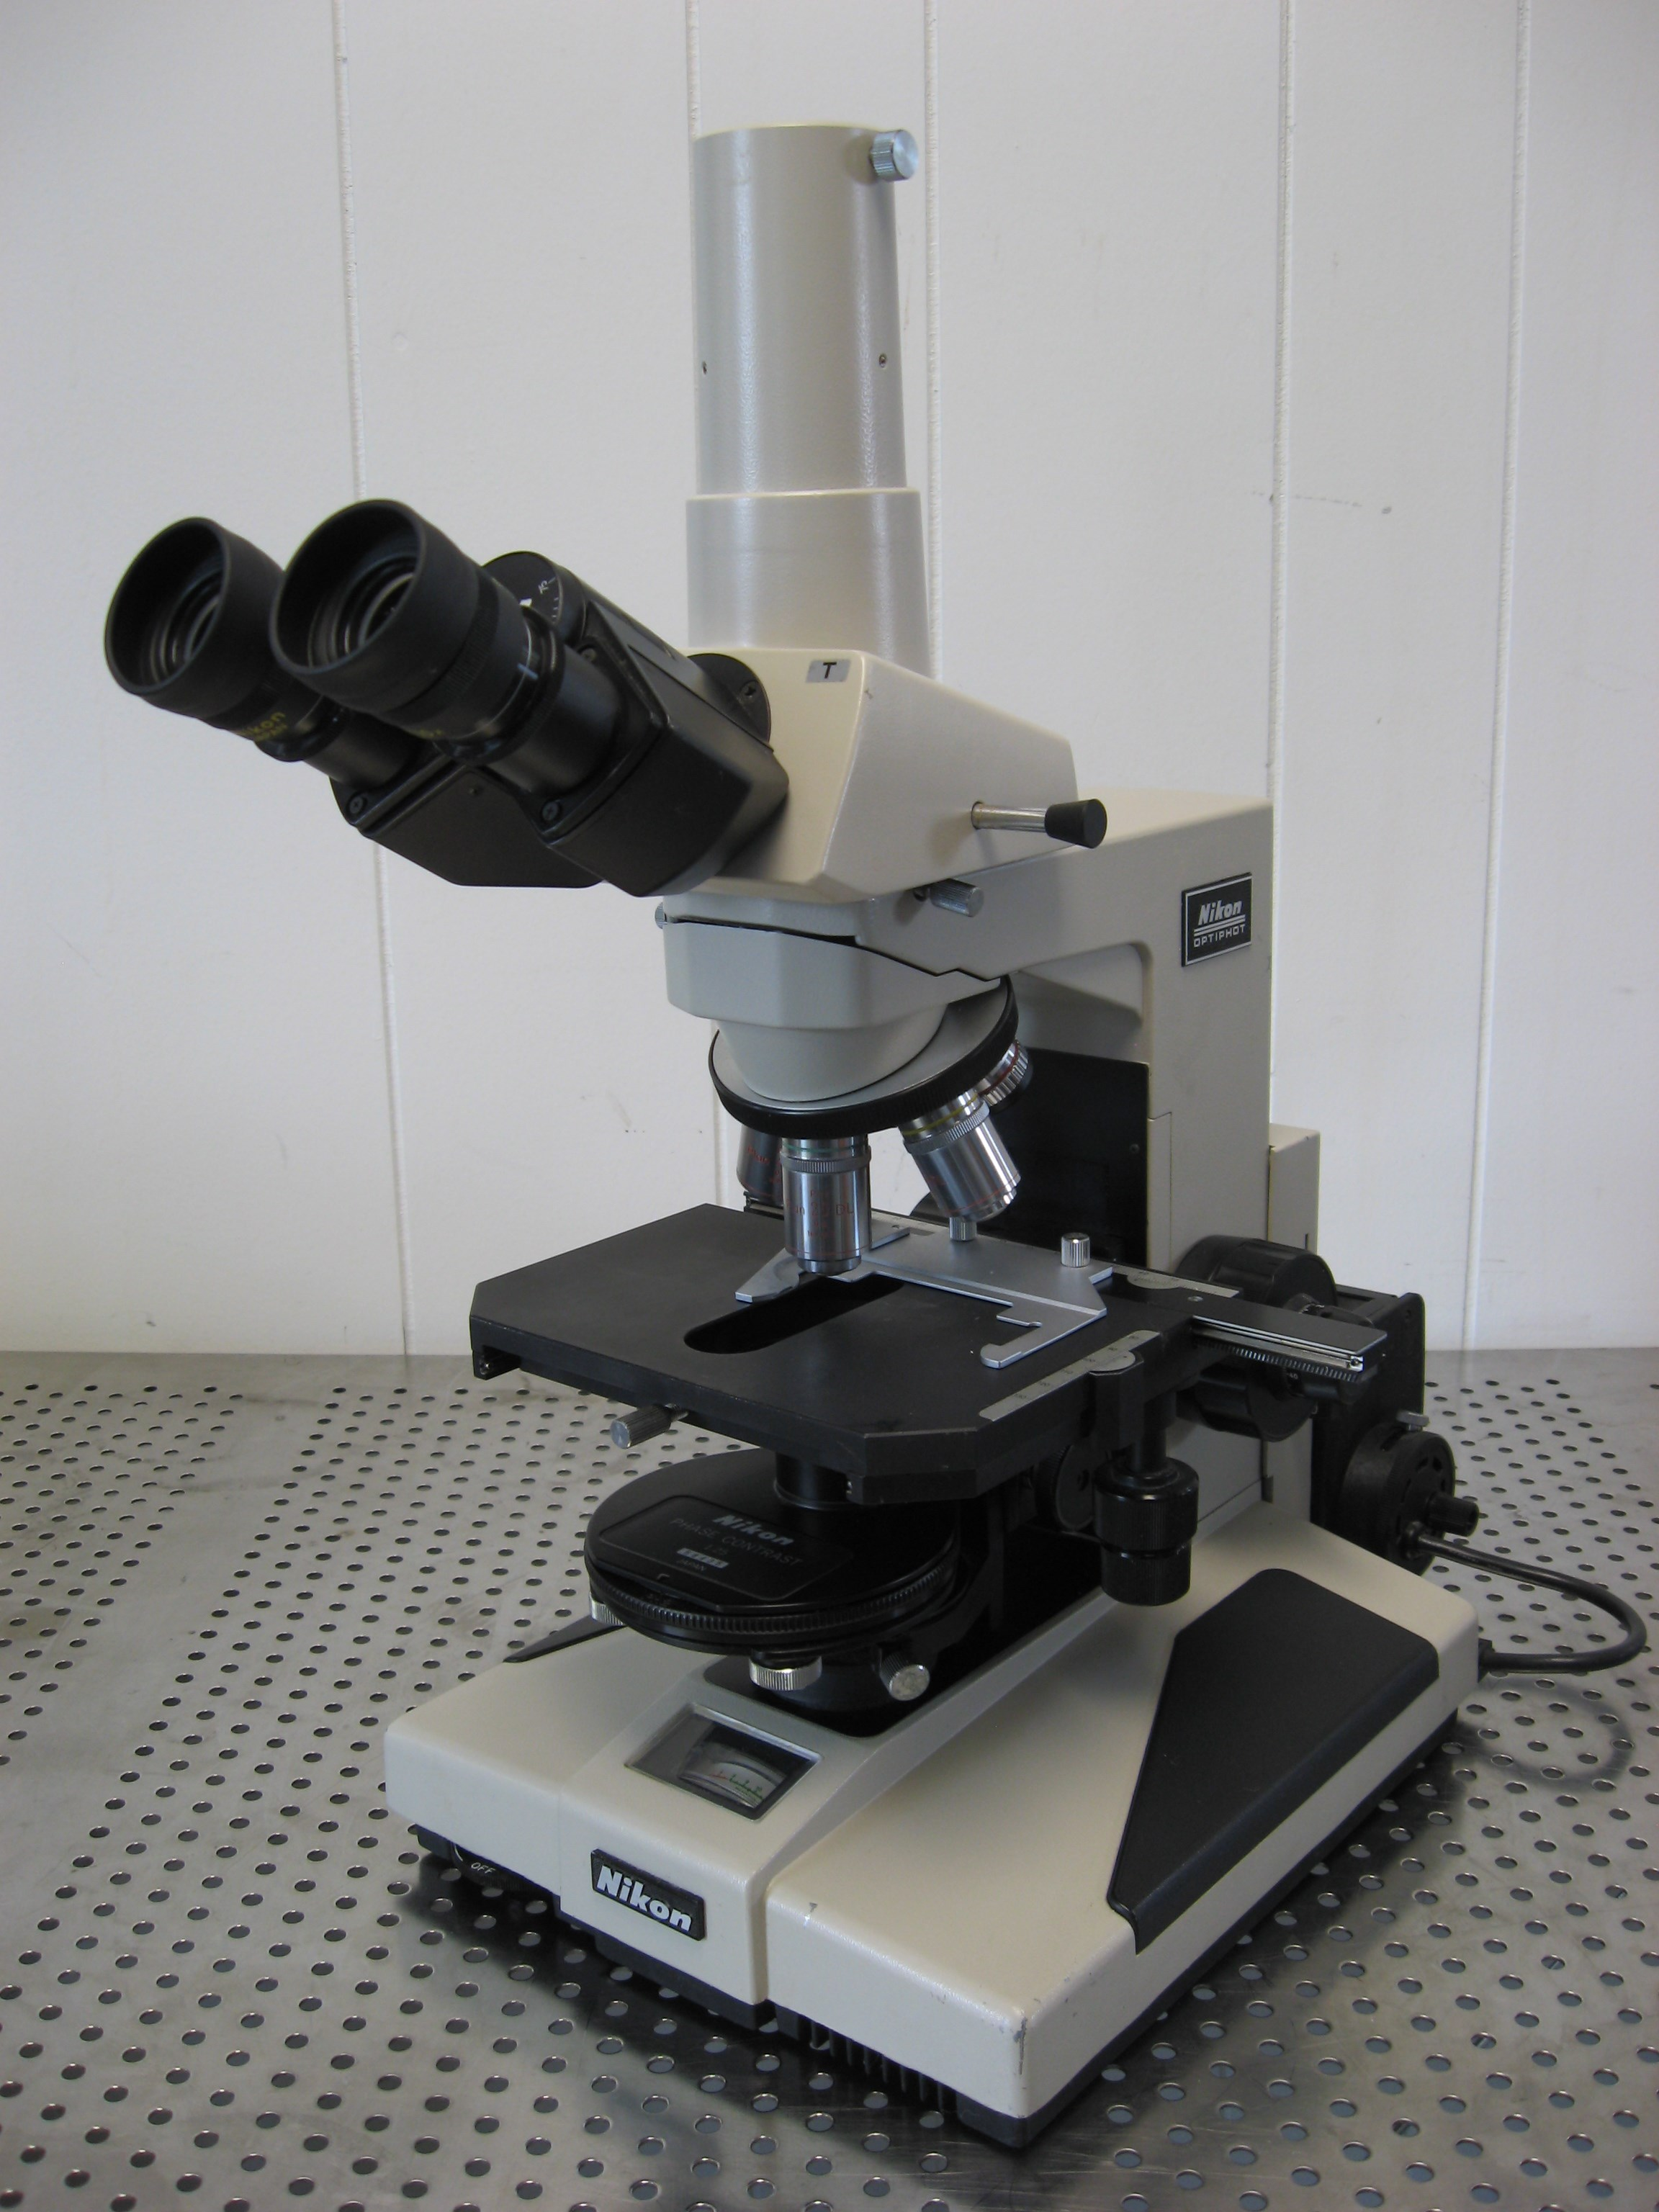
\includegraphics[width=0.35\textwidth]{images/optique.jpg}}
\\
Le microscope optique permet d'observer nos échantillons à l'échelle de la centaine de $\mu m$ ce qui permet de rapidement repérer les défauts les plus gros tels que les pores ou les fissures.
\\

\centerline{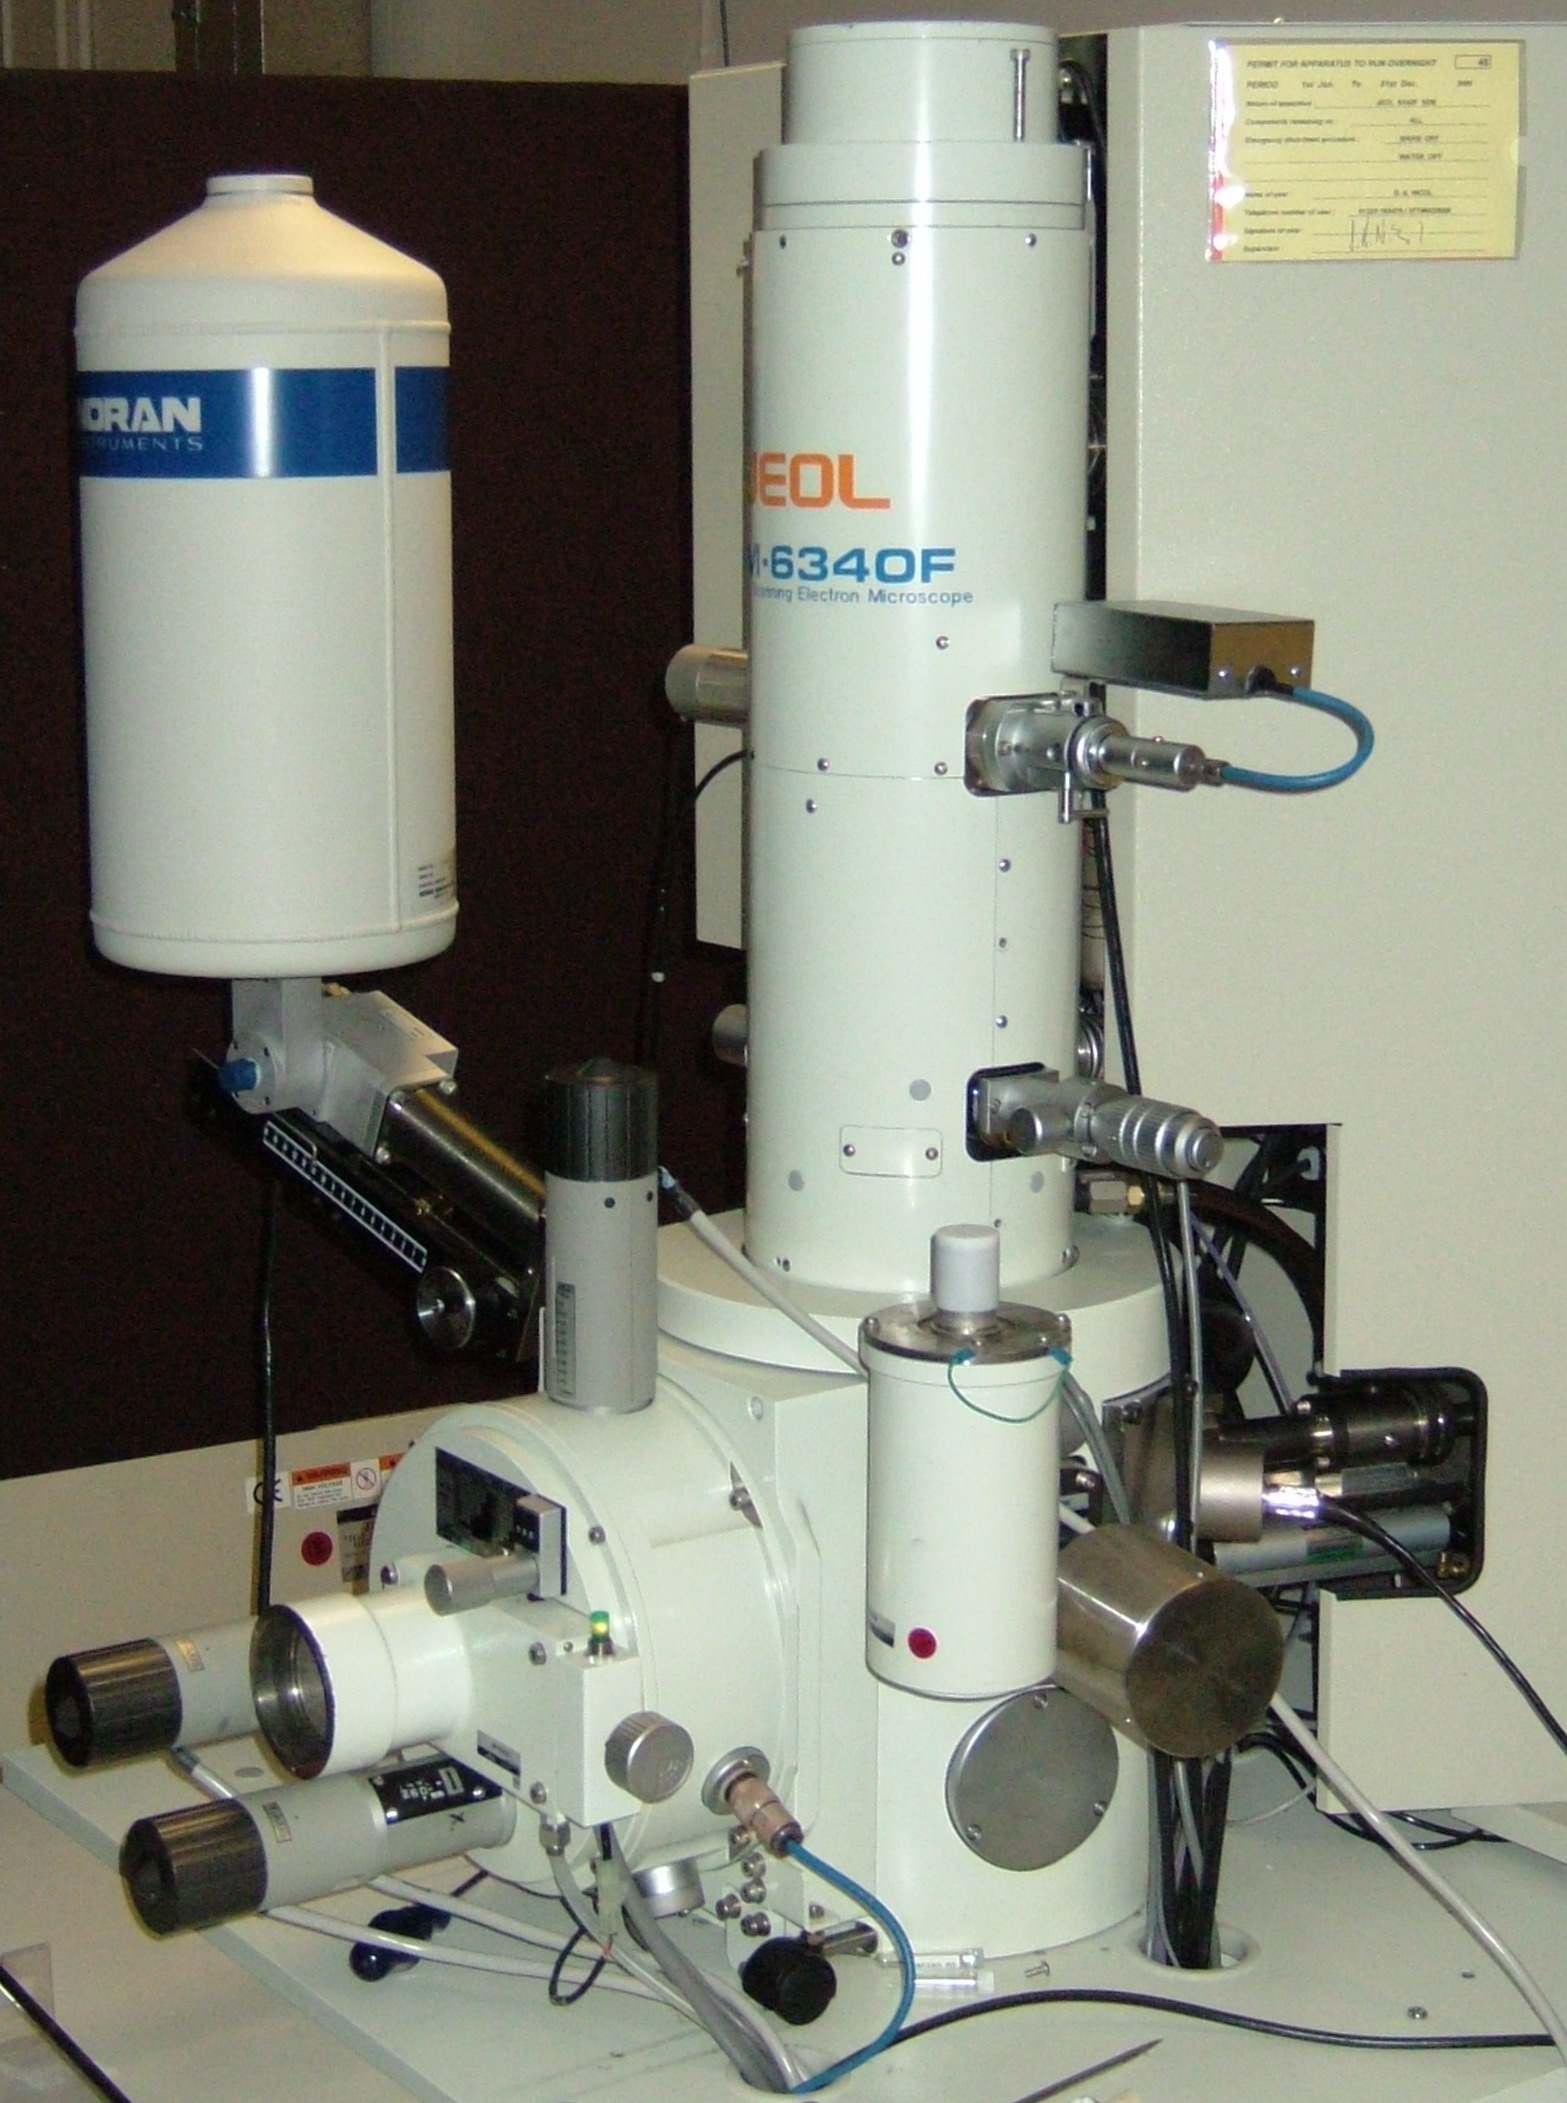
\includegraphics[width=0.4\textwidth]{images/JEOL_JSM-6340F.jpg}}
\\
Des observations au MEB (microscope électronique à balayage) sont réalisées après refroidissement sous haute contrainte. Le microscope optique ne nous permettait pas d'observer l'influence du traitement thermique sur l'agencement des phases $\gamma$ et de $\gamma'$. La résolution du MEB de l'ordre du $\mu m$ nous permet d'observer la phase $\gamma'$ dans la matrice $\gamma$ ainsi que les éventuels agrégats eutectiques. La détection d'électrons rétro-diffusés permet de plus de voir à l'image les phases $\gamma$ et $\gamma'$. En effet les atomes légers de la phase $\gamma'$ sont moins déviés que les atomes plus lourds de la phase $\gamma$. Ainsi les couloirs de matrice $\gamma$ apparaissent en blanc et la phase $\gamma'$ apparaît en noir.
\newpage

